\documentclass[10pt,letterpaper, onecolumn]{article}
%\usepackage[utf8]{inputenc}
\usepackage[T1]{fontenc}    % use 8-bit T1 fonts
\usepackage{graphicx} % Required for the inclusion of images
\usepackage{amsmath} % Required for some math elements 
\usepackage{times}
\usepackage{lipsum} % to be removed later
\usepackage{verbatim}
\usepackage{float}
\usepackage[colorlinks=true, urlcolor=blue, citecolor=blue, linkcolor =blue]{hyperref}       % hyperlinks
\usepackage{enumitem} % to remove space between enum points
% MATH PACKAGES
\usepackage{amsmath,bm}
\usepackage{amssymb}

\usepackage{subfigure}

\usepackage[title]{appendix}

% For subsubsubsection
\usepackage{titlesec}
\setcounter{secnumdepth}{4}
\titleformat{\paragraph}
{\normalfont\normalsize\bfseries}{\theparagraph}{1em}{}
\titlespacing*{\paragraph}
{0pt}{3.25ex plus 1ex minus .2ex}{1.5ex plus .2ex}

% Remove indent for all paragraphs
\usepackage{parskip} 

\usepackage{abstract}
\setlength{\absleftindent}{0mm}
\setlength{\absrightindent}{0mm}

\usepackage{xcolor}
\definecolor{shadecolor}{RGB}{230,230,230}

\usepackage{mdframed}
\mdfdefinestyle{mdfabstract}
{
    backgroundcolor=shadecolor,
    hidealllines=true,
    leftmargin=0.1\textwidth,
    rightmargin=0.1\textwidth
}

\usepackage[%showframe,
top = 1.0in, 
bottom = 1.25in,
footskip = 25pt,
marginparsep = 0pt,
headsep = 0pt]{geometry}

\title{\vspace{-3cm}
\noindent\makebox[\linewidth]{\rule{0.8\textwidth}{2.0pt}} \\ 
\textbf{Level Set Based Image Segmentation} \\
\vspace{-0.30cm}
\noindent\makebox[\linewidth]{\rule{0.8\textwidth}{0.5pt}}}

\author{Ramya Rao Basava\\
Department of Computer Science\\
University of British Columbia, Vancouver}

\date{}

\begin{document}

\maketitle

\textcolor{red}{\textbf{Note: This work is part of my PhD thesis at University of California San Diego and is copyrighted.}}

%===========================================
% Section
%===========================================
\section{Level set function}
One of the first and the most influential work on using Level set methods was introduced by Osher and Sethian \cite{osher1988fronts} which gives numerical solutions to solving problems associated with fronts moving with a curvature dependent speed, using level set functions for curve evolution. The level set function is an implicit, sign-distance function in $n^{\text{th}}$ dimension and its zeroth isocontour represents the moving interface, which is one dimension lower than the level set function dimension. Consider a closed moving interface $\Gamma(t)$ in the domain $\Omega$ and let $\phi(\bm{x},t)$ be a continuous function defined as: 
%
\begin{subequations}
\begin{align}
\phi(\bm{x},t)>0 \quad & \text{if}\  \bm{x} \ \text{is inside} \ \Gamma(t) \\ 
\phi(\bm{x},t)=0 \quad & \text{if}\  \bm{x} \ \text{is on} \ \Gamma(t) \\
\phi(\bm{x},t)<0 \quad & \text{if}\  \bm{x} \ \text{is outside} \ \Gamma(t) 
\end{align}
\label{eqn3.1}
% If label is given here only the main number is refered without the sub parts
\end{subequations}
%
$\phi(\bm{x},t)$ is said to be the level set function of the interface $\Gamma(t)$. 
The motion of this interface is governed by the evolution of the level set function. Some of the important parameters associated with the interface $\Gamma(t)$ can be defined in terms of the level set function as follows:

\noindent Unit outward normal:
%
\begin{equation}
\bm{n} = \frac{\triangledown \phi(\bm{x},t)}{\left\vert \triangledown \phi(\bm{x},t) \right\vert}
\label{eqn:3.2}
\end{equation}
%
Curvature of $\Gamma(t)$:
%
\begin{equation}
\kappa = \triangledown \cdot \bm{n} = \triangledown \cdot \left(  \frac{\triangledown \phi(\bm{x},t)}{\left\vert \bigtriangledown \phi(\bm{x},t) \right\vert} \right)
\end{equation}
%
Area inside $\Gamma(t)$:
%
\begin{equation}
A_{in} = \int_{\Omega} H(\phi(\bm{x},t)) d\bm{x}
\end{equation}
%
Area outside $\Gamma(t)$:
%
\begin{equation}
A_{out} = \int_{\Omega} [1 - H(\phi(\bm{x},t))] d\bm{x}
\end{equation}
%
Length of $\Gamma(t)$:
%
\begin{equation}
L = \int_{\Omega} \delta(\phi(\bm{x},t))
 \left\vert \bigtriangledown \phi(\bm{x},t) \right\vert  d\bm{x}
\end{equation}
%
where $H(\bullet)$ and $\delta(\bullet)$ represent the Heaviside function and Dirac delta 
function defined as follows:
%
\begin{equation}
H(z)=
\begin{cases}
1 \quad       &\text{for } z\geq0   \\
0 \quad       &\text{for } z <0
\end{cases} 
\end{equation}
%
%
\begin{equation}
\delta(z)  = \frac{dH(z)}{dz}
\end{equation}
%

For numerical purposes the regularized version of $H(\bullet)$ and $\delta(\bullet)$ are used in practice. For practical applications the level set function is chosen to be a signed distance function, which is an implicit smooth function and is defined below \cite{osherbook2003level}:
%
\begin{equation}
\phi(\bm{x}) = min(\vert \bm{x} - \bm{x}_I \vert)  \quad \text{for all }  \bm{x}_I  \in \Gamma
\end{equation}
%

The sign distance function also obeys the property of $ \vert \triangledown \phi (\bm{x}) \vert = 1$. 
Example of a signed distance function is shown in figure \ref{fig:3.1}, where the black contour indicates the zero$^{\text{th}}$ level set curve.
%
%
%
\begin{figure}[t] % t - top, b - bottom, h - here
  \begin{center}
    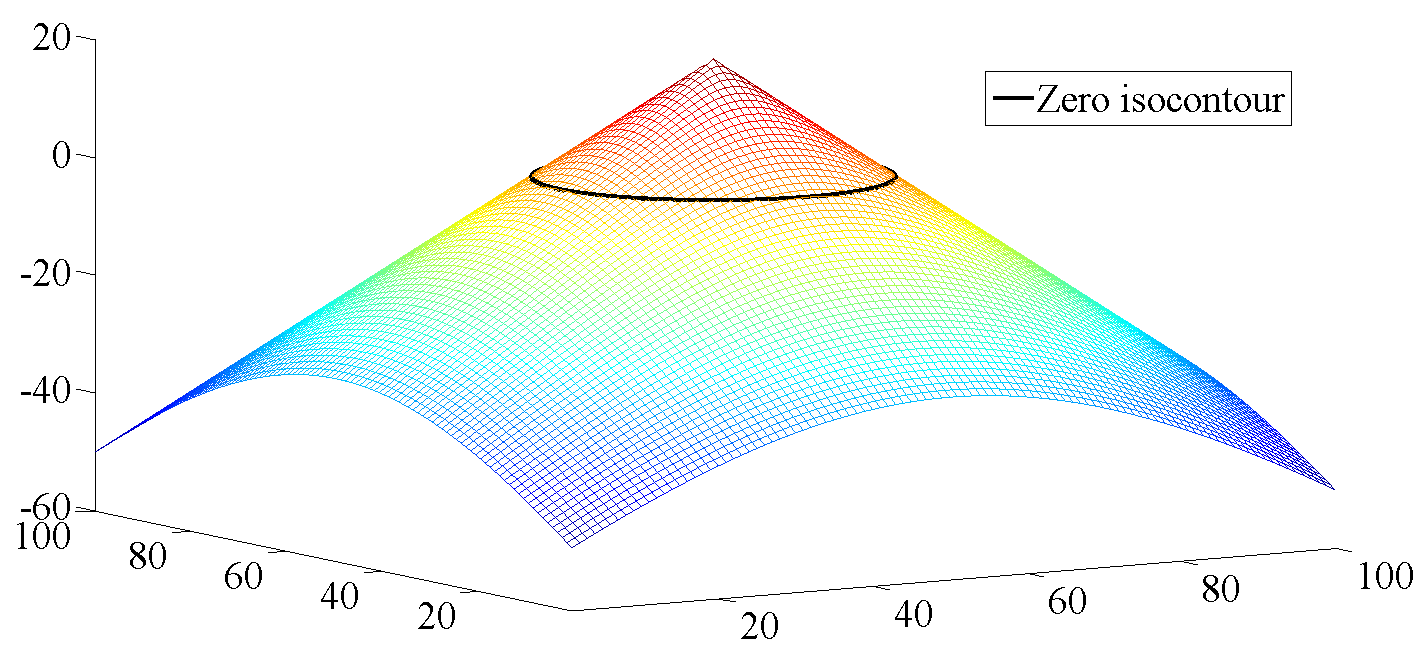
\includegraphics[width=0.7\textwidth,keepaspectratio=1,scale=1]{images/LSisocontour.png}
  \end{center}
  \caption{Signed distance level set function. Black contour represents the zero$^{\text{th}}$ isocontour of the level set function}
  \label{fig:3.1}
\end{figure}
%
%
During numerical time evolution the level set function tends to deviate from a signed distance function which may cause numerical instability. To avoid this, the level set function is re-initialized periodically to make it a signed distance function. Additional re-initialization equation given in \eqref{eqn3.10} should be solved which makes the procedure computationally expensive. In the present work re-initialization has not been required to be done in any of the examples given.
%
%
\begin{align}
&\frac{\partial \psi}{\partial t}  = sign(\phi(\bm{x}, \tau)) (1-\vert \triangledown \psi \vert) \notag \\
&\psi(\bm{x},0) = \phi(\bm{x}, \tau)
\label{eqn3.10}
\end{align}
%
%

In the past two decades level set based methods have been very successfully applied in the field of image segmentation, where the level set function is used for boundary or interface identification. The main advantage of using the level set surfaces in image segmentation is their ability to easily identify topological changes in images, that is, splitting and merging of regions.   



%===========================================
% NEXT SECTION
%===========================================
\section{Active contours without edges (ACWE)}
The ACWE method was proposed by Chan and Vese \cite{chan2001active} and is derived from the piecewise constant Mumford-Shah functional in a level set framework for image segmentation. The following paragraph illustrates this method in the context of segmenting an image which has two distinct intensities - 2 phase segmentation.

 Consider an evolving curve  $\Gamma(t)$ in the domain $\Omega$. Let the image be formed by two regions, 
inside region $R^{in}$ surrounded by the outside region $R^{out}$ as shown in figure \ref{fig:3.2a}. The two regions have approximately piece-wise constant intensities given by
$u_o^{in}$ in $R^{in}$ and $u_o^{out}$ in $R^{out}$, respectively. The aim is to obtain the final boundary
$\Gamma(t)$ such that $u_o(\bm{x}) \in R^{in} \approx u_o^{in}$ and $u_o(\bm{x}) \in R^{out} \approx u_o^{out}$ 
as shown in figure \ref{fig:3.2b}, where $u_o(\bm{x})$
is the pixel intensity at point $\bm{x}$. To achieve this, following ‘fitting’ functional is minimized:
%
\begin{figure}[H]
  \begin{center}
    \subfigure[Initial $0^{\text{th}}$ isocontour of level set function]{\label{fig:3.2a}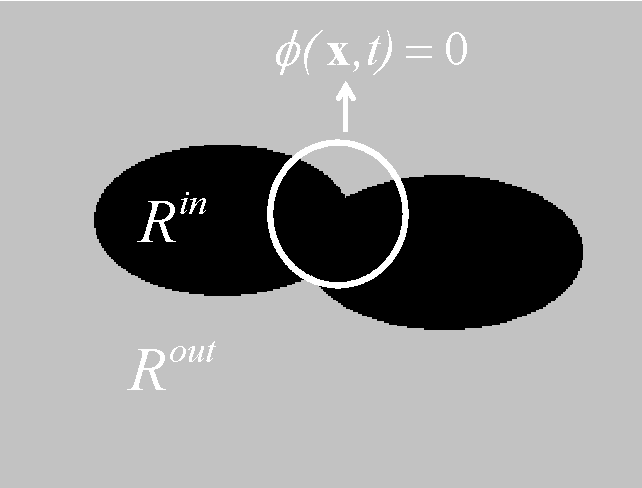
\includegraphics[width=0.49\textwidth,keepaspectratio=1,scale=1]{images/LSinitial_scissored.pdf}} \hfill % default file extension is .eps
% \hfill aligns the figures to page margins of the left and right with space in between the figures
    \subfigure[Final contour obtained after segmentation]{\label{fig:3.2b}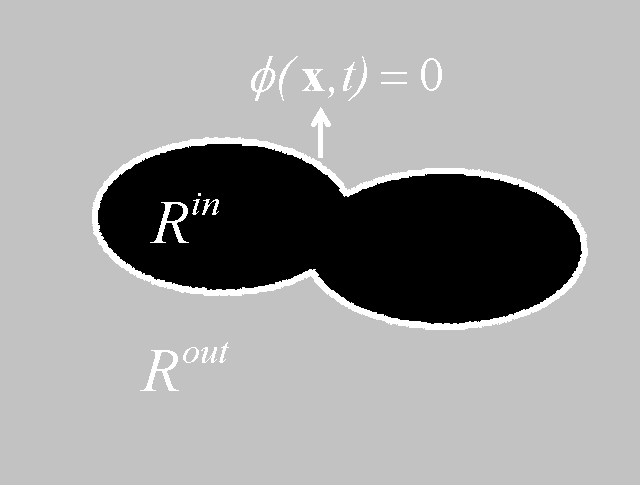
\includegraphics[width=0.49\textwidth,keepaspectratio=1,scale=1]{images/LSfinal_scissored.pdf}}
  \end{center}
  \caption{Two phase (region) segmentation using ACWE method }
  \label{fig:3.2}
\end{figure}
%
%
%----------
%
\begin{align}
\Pi(c_1,c_2,\Gamma) &= \mu \  length(\Gamma) + 
\nu \  Area\ inside (\Gamma) \notag \\
& + \lambda_1 \int_{inside \ \Gamma} 
(u_o(\bm{x}) - c_1)^2 d\bm{x} 
+ \lambda_2 \int_{outside \ \Gamma} 
(u_o(\bm{x}) - c_2)^2 d\bm{x}  
\label{eqn3.11}
\end{align}
%
%
where $\mu$, $\nu$, $\lambda_1$, $\lambda_2$ are non-negative parameters which indicate weights for their respective terms in the above functional. Introducing the level set formulation into the above functional, equation 
\eqref{eqn3.11} can be re-written as:
%
%
\begin{align}
\Pi(c_1,c_2,\phi) &= \mu  \int_\Omega  \delta (\phi(\bm{x}))
\vert \triangledown \phi (\bm{x}) \vert d\bm{x} + 
\nu \int_\Omega  H (\phi(\bm{x})) d\bm{x}  \notag \\
& + \lambda_1 \int_{\Omega} 
(u_o(\bm{x}) - c_1)^2 H (\phi(\bm{x})) d\bm{x} \notag \\
& + \lambda_2 \int_{\Omega} 
(u_o(\bm{x}) - c_2)^2 [1-H (\phi(\bm{x}))] d\bm{x}  
\label{eqn3.12}
\end{align}
%
%
The expressions for the unknowns $c_1$ and $c_2$ can be obtained by minimizing \eqref{eqn3.12} with respect to $c_1$ and $c_2$, respectively, keeping all other variables constant:
%
\begin{equation}
c_1 = \frac{\int_{\Omega}  u_o(\bm{x}) H (\phi(\bm{x})) d\bm{x} }
{\int_{\Omega} H (\phi(\bm{x})) d\bm{x}}
\label{eqn3.13}
\end{equation}
%
%
\begin{equation}
c_2 = \frac{\int_{\Omega}  u_o(\bm{x}) [1-H (\phi(\bm{x}))] d\bm{x} }
{\int_{\Omega} [1-H (\phi(\bm{x}))] d\bm{x}}
\label{eqn3.14}
\end{equation}
%
It can be seen from equations \eqref{eqn3.13} and \eqref{eqn3.14} that $c_1$ represents the average of 
$u_o(\bm{x})$ inside $\Gamma(t)$ and $c_2$ the represents the average of 
$u_o(\bm{x})$ outside $\Gamma(t)$. Minimizing the functional \eqref{eqn3.12} with respect to $\phi$ keeping
$c_1$ and $c_2$ constant, the Euler-Lagrange equations are deduced. In this process, the minimization is parameterized by artificial time $t \geq 0$, which gives the evolution of the level set function and associated boundary conditions as follows:
%
%\begin{subequations}
\begin{align}
&\frac{\partial \phi}{\partial t} = \delta (\phi) \left[ \mu \triangledown \cdot
\left(  \frac{\triangledown \phi}{\vert \triangledown \phi \vert}  \right) - \nu - \lambda_1 (u_o(\bm{x}) - c_1)^2 + \lambda_2 (u_o(\bm{x}) - c_2)^2  \right] \quad \text{in }
\Omega \notag \\ 
& \frac{\delta (\phi)}{\vert \triangledown \phi \vert} 
\triangledown \phi \cdot \bm{n} = 0 \quad \text{on }
\partial \Omega  \notag \\
&\phi(\bm{x},0) = \phi^o(\bm{x}) \quad (\text{given})
\label{eqn3.15}
\end{align}
% If label is given here only the main number is refered without the sub parts
%\end{subequations}
%
%
Here $\Omega$ represents the interior domain of the image and $\partial \Omega$ represents the boundary of the image. As mentioned in the previous section the regularized versions of $H(\bullet)$ and $\delta(\bullet)$ as given below are used 
for numerical implementation. 
\begin{equation}
H_{\varepsilon}(z) = \frac{1}{2} \left[ 1 + \frac{2}{\pi} arctan \left( \frac{z}{\varepsilon} \right) \right]
\label{eqn3.16}
\end{equation}
%
%
\begin{equation}
\delta_{\varepsilon}(z) = \frac{1}{\pi} \left[ \frac{\varepsilon}{\varepsilon^2 + x^2} \right]
\label{eqn3.17}
\end{equation}
%
%
where $\varepsilon$ is a positive parameter. $\varepsilon$ is taken to be equal to 0.5 in all the examples provided in further chapters unless specified. The boundary condition in equation \eqref{eqn3.15} which corresponds to the image boundary does not play a significant role in finding the segmented regions which are in the interior of the image. In all examples in this work a constant term is used for updating $\phi$ near the boundaries. Equation \eqref{eqn3.15} is solved numerically using a semi-implicit scheme, which is detailed in Appendix \ref{Appendix-A}.

%----------------------------------------------------------------
\subsection{Example: Two phase ACWE segmentation}
%----------------------------------------------------------------

This example illustrates the two phase image segmentation using one level set function for the gray scale image shown in figure \ref{fig:3.2}. 
The values of parameters used are $\mu = 100$, $\lambda_1 = 1$, $\lambda_2 = 1$, $\nu = 0$ and $\triangle t = 1$.
The final contour obtained which segments the 2 regions, is shown in figure \ref{fig:3.2b}.


%===========================================
% NEXT SECTION
%===========================================
\section{Extension of ACWE model for multiphase and multichannel segmentation}
\subsection{Multiphase level set method}

The multiphase level set method \cite{vese2002multiphase} is an extension to the 2 phase ACWE formulation described in the previous section. It is a generalized multiphase level set framework to segment images having multiple connected regions (or phases). In this method multiple level set curves are used to segment multiple regions and also triple junctions, without creating any overlap or vacuum in the segmented image. $k$ level set curves can segment up to $2^k$ regions in the image. The union of all the zero isocontours of the level set functions represents the final boundaries of segmentation. 

\subsection{Vector valued image segmentation}
The ACWE model has been extended to the segmentation of multichannel images in
\cite{chan2000active}. A multi-channeled image can be split into multiple channels, which have to be input together for segmentation. Each pixel has a vector as input in a multichannel image. For example a RGB image consists of 3 channels for red, green, blue respectively. Each channel will be a grayscale image. Similarly a CMYK image can be split into 4 channels for cyan, magenta, yellow and black, respectively.

\subsection{Multiphase multichannel segmentation}

The multiphase segmentation can be applied to multichannel images by combining the multiphase and multichannel segmentation methods. A general framework of the functional for an image with $N$ channels, using $n$ level set curves is given by:
%
%
\begin{align}
\Pi (c_p \text{'s}, \phi_k \text{'s}) &= \sum_{k=1}^n \mu_k
\int_{\Omega} \delta (\phi_k) \vert \triangledown \phi_k \vert d\bm{x} \notag \\
&+ \sum_{p=1}^{2^n} \left(   \int_{\Omega_p} \frac{1}{N}
\sum_{i=1}^N \left(\lambda_p^i
(u_o^i(\bm{x}) - c_p^i)^2 \right) d\bm{x}  \right)
\label{eqn3.29}
\end{align}
%
%
where $u_o^i(\bm{x})$ denotes the pixel intensity in the 
$i^{\text{th}}$ channel at point $\bm{x}$ and $c_p^i$
denotes the unknown constant which represents the mean value of intensity in the region $\Omega_p$ of channel
$i$. The corresponding Euler Lagrange equations and expressions for $c_p^i$ can be obtained by minimizing the above functional \eqref{eqn3.29}.

%===========================================
% appendices
%===========================================
\begin{appendices}
\section{Finite difference scheme for ACWE method}
\label{Appendix-A}
Equation \eqref{eqn3.15} for the ACWE method,  is solved numerically using a semi-implicit scheme as given below:

\begin{align}
\frac{\phi_{i,j}^{n+1} - \phi_{i,j}^{n} }{\triangle t} &= 
\delta_\varepsilon (\phi_{i,j}^{n}) \frac{\mu}{h^2} 
\left[ \left( \frac{\phi_{i+1,j}^{n} - \phi_{i,j}^{n+1}}
{\mathbb{A}} \right) 
- \left( \frac{\phi_{i,j}^{n+1} - \phi_{i-1,j}^{n}}
{\mathbb{B} } \right) \right]  \notag \\
&+
\delta_\varepsilon (\phi_{i,j}^{n}) \frac{\mu}{h^2} 
\left[ \left( \frac{\phi_{i,j+1}^{n} - \phi_{i,j}^{n+1}}
{\mathbb{C}}  \right)
- \left( \frac{\phi_{i,j}^{n+1} - \phi_{i,j-1}^{n}}
{\mathbb{D} } \right) \right] \notag \\
&+
\delta_\varepsilon (\phi_{i,j}^{n})
\left[ -\nu -\lambda_1 (u_{o,i,j} - c_1(\phi_n))^2 +  \lambda_2 (u_{o,i,j} - c_2(\phi_n))^2 \right]
\end{align}
where
%
%
\begin{subequations}
\begin{align}
\mathbb{A} &= \sqrt{ \left(  \frac{\phi_{i+1,j}^{n} - \phi_{i,j}^{n}}{h} \right)^2 
       + \left( \frac{\phi_{i,j+1}^{n} - \phi_{i,j-1}^{n}}{2h}  \right)^2 } \\
\mathbb{B} &= \sqrt{ \left(  \frac{\phi_{i,j}^{n} - \phi_{i-1,j}^{n}}{h} \right)^2 
       + \left( \frac{\phi_{i-1,j+1}^{n} - \phi_{i-1,j-1}^{n}}{2h}  \right)^2 } \\
\mathbb{C} &= \sqrt{ \left(  \frac{\phi_{i+1,j}^{n} - \phi_{i-1,j}^{n}}{2h} \right)^2 
       + \left( \frac{\phi_{i,j+1}^{n} - \phi_{i,j}^{n}}{h}  \right)^2 } \\
\mathbb{D} &= \sqrt{ \left(  \frac{\phi_{i+1,j-1}^{n} - \phi_{i-1,j-1}^{n}}{2h} \right)^2 
       + \left( \frac{\phi_{i,j}^{n} - \phi_{i,j-1}^{n}}{h}  \right)^2 }
\end{align}
\end{subequations}
%
$h$ is the spacing between the pixels in the image, which is the same in both $x$ and $y$ directions and 
$\triangle t$ is the time step increment.

\end{appendices}






\bibliographystyle{plain}
\bibliography{references} 

\end{document}
